\documentclass[thesis.tex]{subfile}
\begin{document}
\chapter{TurtleBot Platform} \label{ch:Hardware Platform}
This chapter describes the hardware platform developed for use with this thesis. A matching simulation model was developed in the Gazebo simulator~\cite{Koenig}.

\section{TurtleBot}
The TurtleBot platform~\cite{TurtleBot} was developed by the Open Source Robotics Foundation, Inc. as an open source hardware platform for use as a low cost, educational mobile robotics platform. We used a combination of the TurtleBot 2 and 2e specifications. The TurtleBot 2e uses a single board computer rather than a netbook, and we used the Avnet ZedBoard~\cite{ZedBoard} for this purpose. However, the 2e switches to the Orbbec Astra camera, but we instead chose to stay with the Microsoft Kinect used in the TurtleBot 2 specification. We chose to do this because the Kinect camera hardware and software is much more established, is cheaper, and much work, like that of \textcite{ganganath2012mobile, biswas2012depth, cunha2011using} have shown that the Kinect is a legitimate tool for localization tasks.

\subsection{Basic Features}
The TurtleBot consists of three main components: the Kobuki mobile base manufactured by Yujin Robot~\cite{Kobuki}, the ZedBoard, and the Microsoft Kinect camera. We have also added a USB hub and an Asus WiFi router to allow for the use of more peripherals and wireless networking. These are necessary because the ZedBoard does not have this functionality built in, unlike the netbook that is suggested for the TurtleBot 2 platform.

With these three components combined, the TurtleBot is a very simple mobile robot with a connected computer and camera for sensing. However, one of the main reasons the TurtleBot is such a compelling platform is its use of \gls{ros}.

\subsection{ROS Interface}
One reason the TurtleBot platform was chosen is because it was designed for use with \gls{ros}~\cite{TurtleBotWiki}. This makes it very easy to write new software for the robot, and lots of the ``heavy lifting" software is made available alongside the platform specification. All of this is open source as well, another strong argument in favor of using it.

\gls{ros} is not a true operating system like the name would imply. It is much more correctly described as a set of libraries and tools that are designed for use in robotics applications. It provides a robust set of communication protocols to allow different software components, called \glspl{node}, to interact with each other. Additionally, there are many existing, open source \gls{ros} packages that can be built upon without having to start from scratch.

\subsection{Controls} \label{sec:controls}
One example of using pre-existing software from the \gls{ros} repositories is control and navigation of the Kobuki base. Writing the control system for a mobile robot would normally be a complex and time consuming task. Because the TurtleBot uses \gls{ros}, we were able implement a known control system very quickly and move on with other research.

\subsubsection{Kobuki Base}
The Kobuki has a very simple control system made up of four \glspl{node}~\cite{KobukiControl}. These four \glspl{node} are the velocity smoother, safety controller, command multiplexer, and the hardware driver. There are three different ways of sending movement commands to the Kobuki: a navigation function, keyboard teleoperation, and Android phone teleoperation. The structure of these nodes and inputs is shown in \cref{fig:kobuki_control}.

\begin{figure}[htbp]
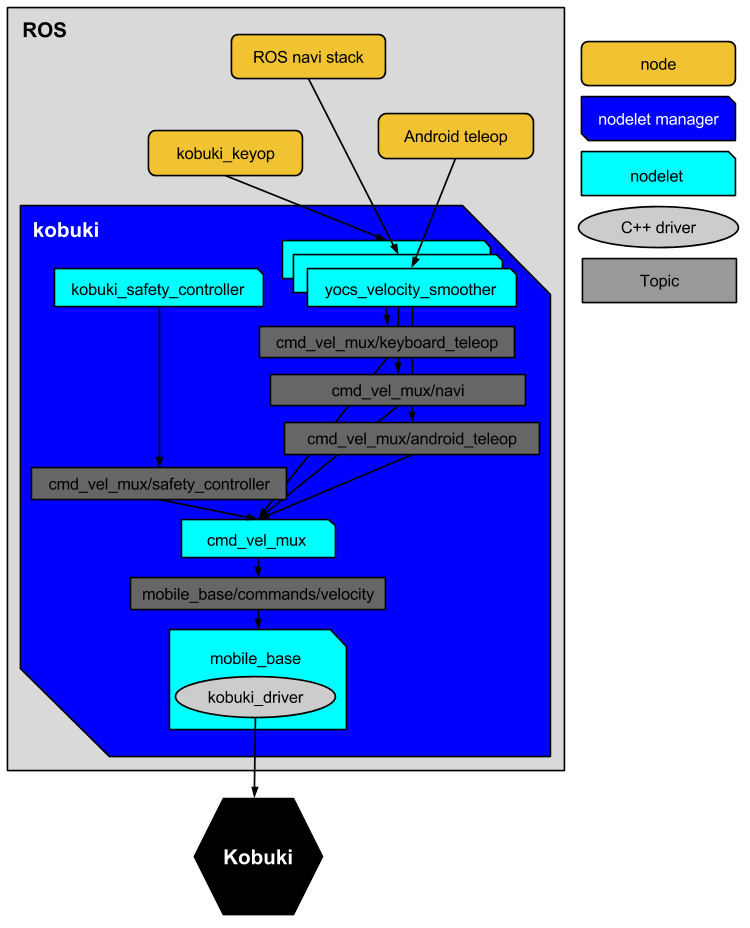
\includegraphics[width=\textwidth, keepaspectratio]{kobuki_control}
\caption[Overview of the Kobuki control system]{Overview of the Kobuki control system, from~\cite{KobukiControl}}
\label{fig:kobuki_control}
\end{figure}

The velocity smoother sits in between these three different input modes and the command multiplexer. It applies robot-specific velocity and acceleration limits to the received commands before republishing them to the multiplexer. The multiplexer selects which of the three possible input commands should be active based on a defined hierarchy. The safety controller watches for cliffs and impacts and always overrides any other navigation input. Finally the multiplexer outputs a final command which is translated by the hardware driver.
 
\subsubsection{Navigation}
For navigation and path planning, both in the real world and simulations, we used the \gls{ros} Navigation Stack~\cite{ros_navigation}. This allows for an intelligent path planning system to be implemented quickly and easily. The Navigation Stack contains both a local and global planner which coordinate to effectively reach the goal. 

\Cref{fig:navigation_stack} shows the full outline of the navigation stack and its nodes. For this thesis, minimal path planning and navigation functions were needed so almost no modifications were made. The only major change from this outline is that no static world map was used, and therefore there is no map server.

\begin{figure}[htbp]
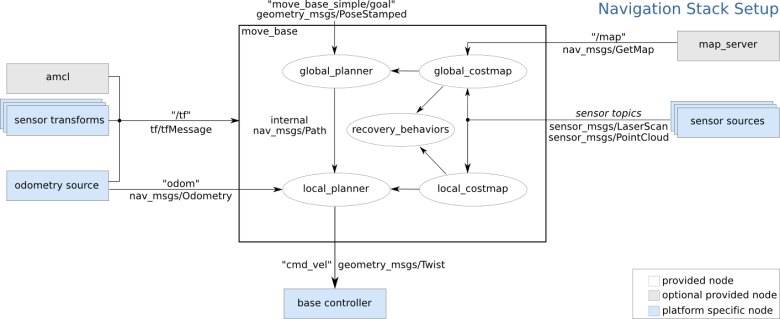
\includegraphics[width=\textwidth, keepaspectratio]{navigation_stack}
\caption[Overview of the \gls{ros} Navigation Stack]{Overview of the \gls{ros} Navigation Stack, from~\cite{NavigationStack}}
\label{fig:navigation_stack}
\end{figure}

\section{ZedBoard}
The ZedBoard is a single board computer featuring the Xilinx Zynq-7000 All Programmable System on a Chip. This was chosen as the main board for this project due to its low cost, low power requirements, and the Zynq chip. The Zynq chip contains both an ARM processor and a Xilinx \gls{fpga}, making it an ideal choice for mobile robotics application which interface extensively with hardware.
 
Because the ZedBoard has an ARM processor, the standard flavors of Ubuntu, the primary operating system for \gls{ros} cannot be installed. Instead, we used Linaro 14.12. Linaro is an embedded Linux development group, and they produce both toolchains and Ubuntu-based operating systems for use on embedded platforms. Linaro 14.12 was chosen because it is the last version of Linaro to be based on Ubuntu Trusty 14.04, which is required for \gls{ros} Indigo Igloo, which is the version of \gls{ros} that this research uses.

With Linaro installed, the ZedBoard acts like a very typical Ubuntu system, and for the casual user would be non-distinguishable. The apt service works as normal, only with limited packages since not all are available in a version compiled for ARM. \gls{ros} however can be installed via apt in the standard way without issues.

%TODO could justify zedboard vs notebook

\end{document}